\chapter{Kontext}

\section{Testování softwaru při vývoji}
Při vývoji softwaru je vhodné vyvíjený software neustále testovat. Software lze testovat
více způsoby, ale cílem testů je vždy otestovat některý z~důležitých kvalitativních
atributů, jako je například korektnost nebo výkon.

Pro testování korektnosti se obvykle používají unit testy. Jedná se většinou o~krátké testovací
funkce, které kontrolují, jestli se testovaný kód chová požadovaným způsobem. Zjišťují tedy ,jestli
kód na zadaný vstup vrátí očekávaný výstup. Ke~kódu, který není aktuálně vyvíjen, se obvykle nemění
ani unit testy.  Proto když se mění části kódu kolem již takto hotové části, tak unit testy stále průběžně sledují
korektnost tohoto již hotového kódu. Zdali je kód korektní se pomocí unit testů zjistí velmi jednoduše.
Kód je korektní, pokud vrátil očekávaný výstup a pokrytí kódu unit testy je dostatečné.

Testování výkonu obvykle probíhá tak, že se použije nějaký vhodný měřící framework.
Obvyklé frameworky pro měření výkonu mají vlastní pravidla, jak se mají označit metody, které
se mají měřit. Tyto frameworky umožňují měřit výkon softwaru podle různých metrik. Mezi tyto metriky
se řadí čas, propustnost a~například spotřeba paměti. Výsledky měření frameworky umí obvykle zaznamenat jak do~strojově
čitelného formátu, tak do formátu čitelného pro člověka. Výsledek měření je ale pouze sada čísel, kde
jsou ke~jménům testovaných metod přiřazeny naměřené hodnoty.

\begin{figure}[!ht]
    \centering
    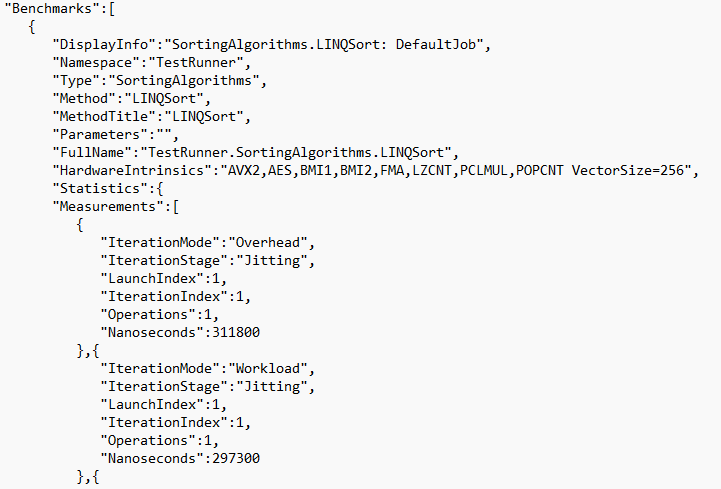
\includegraphics[width=0.92\textwidth]{../img/BenchmarkDotNET-json.png}
    \caption{Příklad části výstupu frameworku BenchmarkDotNET}
\end{figure}

Výsledky testování výkonu se tedy musejí vyhodnocovat tak, že se podrobně prozkoumá výsledná sada čísel.
Oproti testování korektnosti, kdy test projde nebo neprojde, je testování výkonu výrazně složitější.
Pohledem na samostatnou sadu dat se nedá určit, zdali je software dostatečně rychlý. Aby bylo možné
ze~sady určit něco vypovídajícího, bylo by možné stanovit pevný limit výkonnosti.
Tento přístup nemusí být vypovídající při dlouhodobém vývoji
a~při hodnotách hluboko pod limitem. Proto je vhodné, aby se datové sady, které testovací framework produkuje,
porovnávaly mezi sebou. Porovnáním sad je totiž možné zjistit, jestli nedošlo k~významným změnám výkonu
při~vývoji od~předchozí verze. Frameworky samotné však tuto možnost obvykle nemají.

\section{Průběžná integrace}
Při vývoji softwaru se často používají nástroje pro automatizování některých činností.
Obvykle se automatizují činnosti jako jsou správa verzí, spouštění testů a jejich vyhodnocování.

Pro správu verzí při vývoji softwaru se obvykle používá nástroj git.
Git je vhodný i pro práci ve velkých týmech.
Umožňuje totiž členění projektu do větví. Každá větev je vhodná pro vývoj samostatné části aplikace.
Následným spojováním větví pak dochází k propojení větších funkčních celků aplikace, které byly vyvinuty v jednotlivých větvích.
Nástroj si formou pamatování si změn udržuje přehled o průběžných verzích a provedených změnách.
Nástroj je možné ovládat jednoduchými příkazy z příkazové řádky.
Je to tedy nástroj, který je možné ovládat ze skriptů.

Nástroj git umí jednoduše zprostředkovat průběžnou integraci (continuous integration). Průběžná integrace umožňuje uživateli dělat automatizované
kroky při nahrávání nových verzí do~větve nebo při spojování větví. Při průběžné integraci tedy jde o~spouštění
skriptu při některé ze zmíněných událostí. V rámci průběžné integrace je možné testovat software pomocí unit testů
i~benchmarků pro měření výkonu. Dále je možné použít jakékoli jiné příkazy příkazové řádky.
Do průběžné integrace je tedy možné jednoduše zapojit téměř jakoukoli konzolovou aplikaci.

\section{Scénář}

Programátor se rozhodne naprogramovat si své vlastní softwareové dílo. Z~tohoto softwareového díla
časem přestane být malý projekt. Porgramátor tedy usoudí, že je zapotřebí udržovat kvalitu kódu.
Vytvoří si tedy unit testy s~dostatečným pokrytím, aby byl schopen udržovat korektnost napsaného kódu.
Začne používat nějaký verzovací nástroj například Git a vytvoří si skript pro průběžnou integraci.
V~rámci této průběžné integrace bude pomocí unit testů s~každou novou verzí udržovat průběžná korektnost.

Dalším z~aspektů kvality kódu, které by chtěl udržovat je výkon. Programátor s~využitím nějakého frameworku pro~měření výkonu začne měřit výkon svého kódu.
Měření výkonu se trochu podobá unit testům. U~měřících frameworků jako je BenchmarkDotNET nebo JMH se vytvoří specializované měřící metody,
které se podobají unit testovacím metodám z~unit testovacích frameworků jako je například JUnit.
Tyto měřící metody, ale změří pouze číslo a~jednotku, která nevypovídá o~změně výkonu oproti jiné verzi.
Pokud chce programátor výkon udržovat potřebuje vyhodnotit právě tuto změnu.

Programátor tedy musí vzít výsledky měření aktuální verze a výsledky měření referenční verze vůči které chce
změnu výkonu vyhodnocovat a sám výsledky porovnat. Porovnání výsledků měření nemusí být možné pouhým Pohledem
na sady číselných dat. Pravděpodobně si budou hodnoty hodnoty obou sad podobné. Obzvlášť pokud změna bude příliš málo výrazná.
Proto by musel programátor nejprve číselná data nějakým způsobem sám zpracovat. Ze zpracovaných dat by pak pro každou měřeou metodu
kódu musel vyhodnotit zda-li došlo k výrazné změně výkonu, které by se měl dále věnovat.

PerfEval by měl být nástroj, který řeší programátorův problém. Měl by to být nástroj, který bu měl pomoci
z~naměřených datových sad vyhodnotit změnu výkonu a výrazné změny hlásit. Taktéž by mu nástroj měěl být schopen
udržovat výkon průběžně, a~proto by mělo být možné jej použít v~průběžné integraci obdobným způsobem jako frameworky
pro psaní unit testů.

Vyvíjený nástroj PerfEval byl při vývoji směřován k tomu, aby uspokojil potřeby zmíněného programátora.
Vyhodnocování výkonnostních testů se tedy provádí pomocí konzolové aplikace, která se ovládá pomocí
příkazů a~argumentů. Tento design byl zvolen zejména kvůli tomu, aby se nástroj používal co nejvíce
jako spouštění unit testů v~rámci průběžné integrace.
